%%%%%%%%%%%%%%%%%%%%%%%%%%%%%%%%%%%%%%%%%%
% Engineering problems / LaTeX Template
%		Semester 6
%		Institut d'Optique Graduate School
%%%%%%%%%%%%%%%%%%%%%%%%%%%%%%%%%%%%%%%%%%
%	6N-IntNum-BlocCamera	/ Industrial Sensor
%%%%%%%%%%%%%%%%%%%%%%%%%%%%%%%%%%%%%%%%%%
%
% Created by:
%	Julien VILLEMEJANE - 16/jul/2024
% Fichier.sty modifié pour changer la police de caractère
%	
%
%%%%%%%%%%%%%%%%%%%%%%%%%%%%%%%%%%%%%%%%%%
% Professional Newsletter Template
% LaTeX Template
% Version 1.0 (09/03/14)
%
% Created by:
% Bob Kerstetter (https://www.tug.org/texshowcase/) and extensively modified by:
% Vel (vel@latextemplates.com)
% 
% This template has been downloaded from:
% http://www.LaTeXTemplates.com
%
% License:
% CC BY-NC-SA 3.0 (http://creativecommons.org/licenses/by-nc-sa/3.0/)
%
%%%%%%%%%%%%%%%%%%%%%%%%%%%%%%%%%%%%%%%%%

\documentclass[a4paper,11pt,titlepage]{article} % The default font size is 10pt; 11pt and 12pt are alternatives

%%%%%%%%%%%%%%%%%%%%%%%%%%%%%%%%%%%%%%%%%%%%%%%%%%%%%%%%%%%%%%%%%%%%%%%%%%%%%%%%%%%%%%%%%%%%%%%%%%%%%%%%%%%%%%%%%%%%%%%%%%%%%%%%%%%%%%%%%%%%%%%%%%%%%%%%%%%%%%%%%%%%%%%%%%%%%%%%%%%%%%%%%%%%%%%%%%%%%%%%%%%%%%%%%%%%%%%%%%%%%%%%%%%%%%%%%%%%%%%%%%%%%%%%%%%%
\usepackage{opto_elec_villemejane}

%%%%%%%%%%%%%%%%%%%%%%%%%%%%%%%%%%%%%%%%%%%%%%%%
%%%%%%%%%%%%%%%%%%%%%%%%%%%%%%%%%%%%%%%%%%%%%%%%
\begin{document}



% Page de garde
\begin{titlepage}

\begin{center}
	\begin{minipage}{2.5cm}
	\begin{center}
		
\includegraphics[width=8cm]{images/Logo-LEnsE.png}
	\end{center}
\end{minipage}\hfill
\begin{minipage}{10cm}
	\begin{center}
	\textbf{Institut d'Optique Graduate School }\\[0.1cm]
    \textbf{Interfaçage Numérique}


	\end{center}
\end{minipage}\hfill


\vspace{4cm}


{\huge \bfseries \textsc{Interfaçage Numérique}} \\[0.5cm]
{\large \bfseries Travaux Pratiques} \\[0.2cm]
Semestre 6

\vspace{1.2cm}
% Title
\rule{\linewidth}{0.3mm} \\[0.4cm]
{ \huge \bfseries\color{violet_iogs} Chaine d'acquisition d'une image \\ Manipulation d'images\\[0.4cm] }
\rule{\linewidth}{0.3mm} \\[0.8cm]

2 séances

\bigskip

\begin{center}
	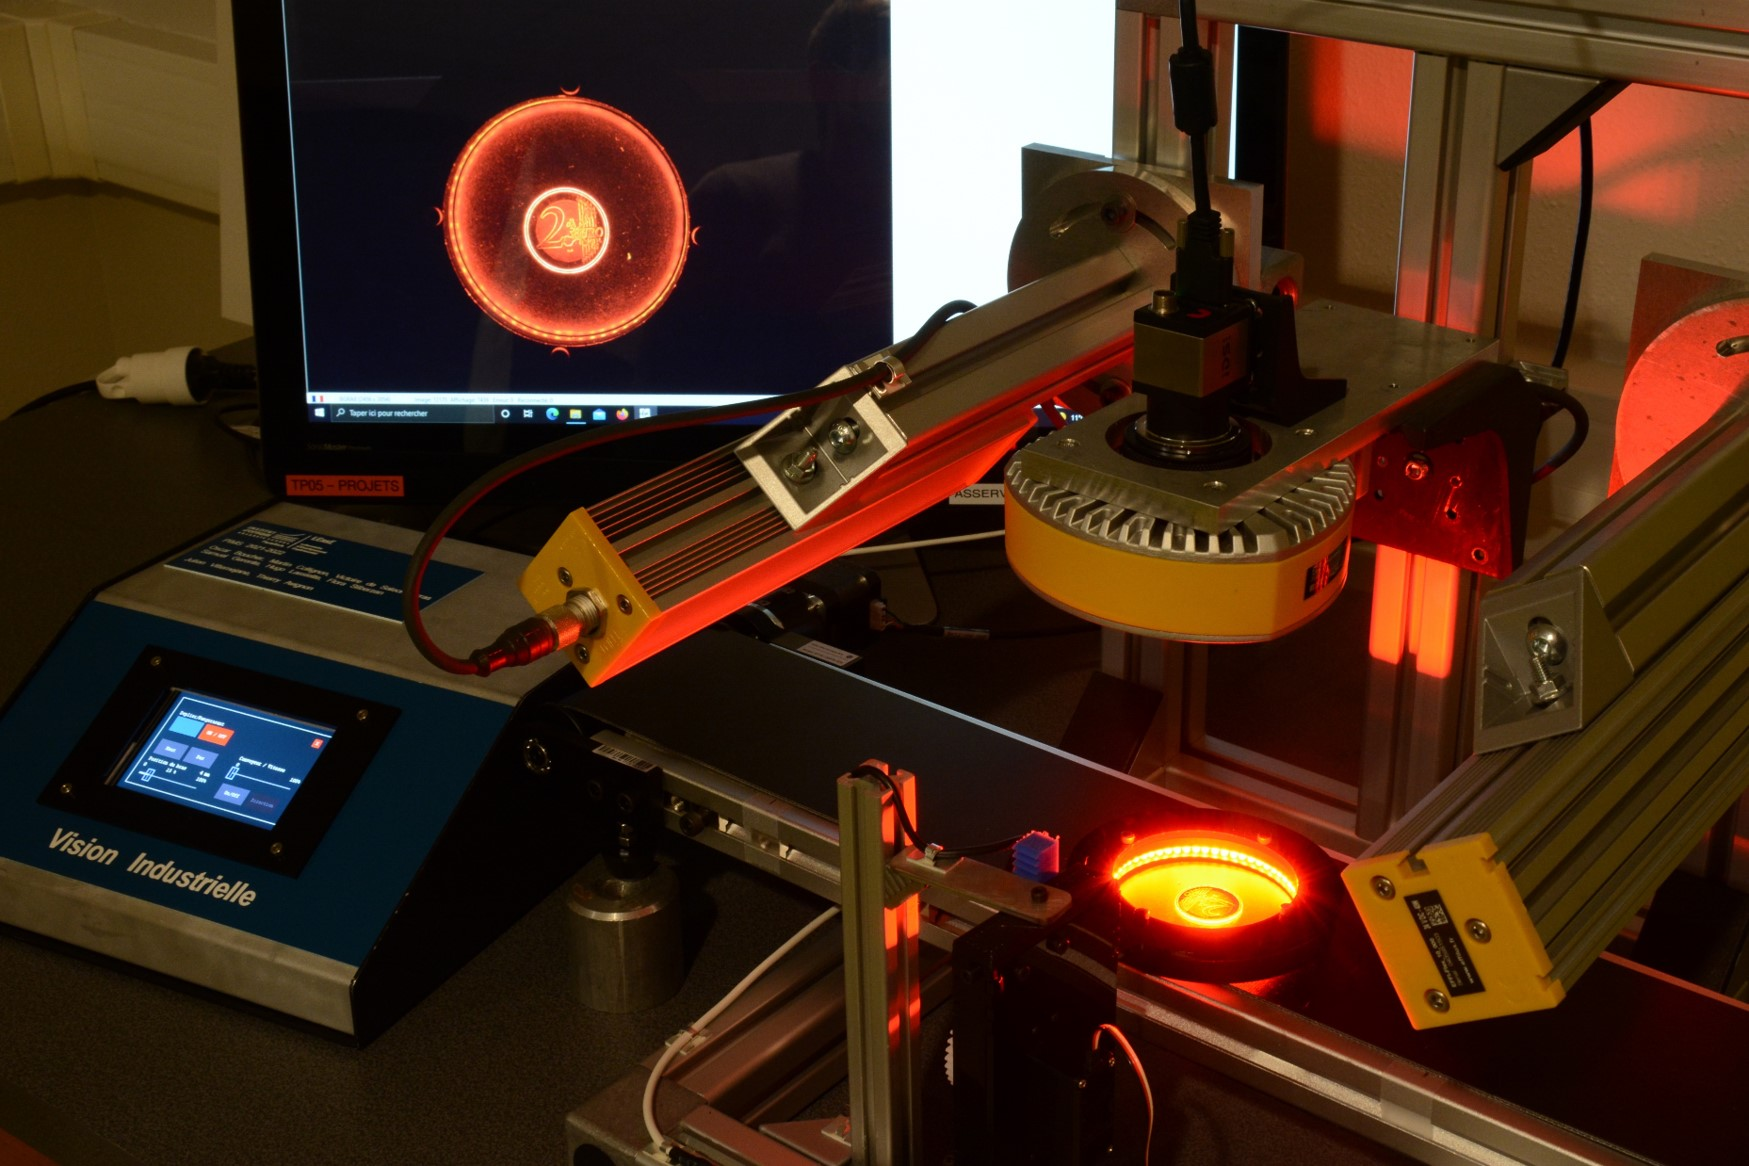
\includegraphics[width=0.5\textwidth]{images/camera_vi.jpg}
\end{center}

\bigskip

\vfill

\textit{Ce sujet est disponible au format électronique sur le site du LEnsE - https://lense.institutoptique.fr/ dans la rubrique Année / Première Année / Interfaçage Numérique S6 / Bloc 2 Caméra, Images et Interfaces / Caméra}

% Bottom of the page
%{\textbf{\large {Année universitaire} 2024-2025}}

\end{center}
\end{titlepage}

\newpage
\strut % empty page


%%%%%%%%%%%%%%%%%%%%%%%%%%%%%%%%%%%%%%%%%%%%%%%%
%%%%%%%%%%%%%    Intro
\newpage
\pagestyle{empty}

\begin{minipage}[c]{.25\linewidth}
	
\includegraphics[width=5cm]{images/Logo-LEnsE.png}
\end{minipage} \hfill
\begin{minipage}[c]{.4\linewidth}

\begin{center}
\vspace{0.3cm}
{\Large \textsc{Interfaçage Numérique}}

\medskip

6N-047-SCI \qquad \textbf{\Large Bloc Caméra}

\end{center}
\end{minipage}\hfill

\vspace{0.5cm}

\noindent \rule{\linewidth}{1pt}

{\noindent\Large  \rule[-7pt]{0pt}{30pt} \textbf{Chaine d'acquisition d'une image et manipulation d'images avec OpenCV}}

\noindent \rule{\linewidth}{1pt}

\bigskip

%%%%%%%%%%%%%%%%%%%%%%%%%%%%%%%%%%%%%%%%%%%%%%%%
%%%%%%%%%%%%%    Objectifs

\section{Objectifs du bloc}

L'objectif principal de ce bloc est de découvrir les \textbf{différents paramètres impactant la qualité d'une prise d'image par une caméra} dans un environnement industriel ainsi que la \textbf{manipulation d'images numériques}, à l'aide de la bibliothèque \textbf{OpenCV}.

On s'intéressera à l'impact du \textbf{temps d'intégration}, de la \textbf{résolution} de la caméra et de l'\textbf{éclairage} (couleur et intensité) de la scène et des objets sur l'image résultante. 


\noindent \rule{\linewidth}{1pt}

\medskip

%%%%%%%%%%%%%%%%%%%%%%%%%%%%%%%%%%%%%%%%%%%%%%%%
%%%%%%%%%%%%%    A A V

À l'issue des séances de TP concernant le bloc sur les caméras industrielles et la manipulation d'images, les étudiant$\cdot$es seront capables de~:

\begin{itemize}
	\item paramétrer le temps d'exposition en fonction de l'intensité lumineuse pour \textbf{obtenir une image d'une qualité exploitable}
	\item utiliser des outils d'analyse (histogramme notamment) pour \textbf{améliorer numériquement} la qualité d'une image (contraste, luminosité...)
	\item \textbf{manipuler une image numérique} à l'aide de la bibliothèque \textsl{OpenCV}
	% \item \textbf{extraire des primitives} de bas niveau dans une image.
\end{itemize}

\noindent \rule{\linewidth}{1pt}


\textit{Cette étude sera complétée par un TP plus détaillé sur les bruits associés à l'utilisation des caméras CMOS en 2ème année du cycle ingénieur à Palaiseau.}

\textit{Des cours et des projets autour du traitement d'images sont également proposés dans les prochaines années de formation, quelque soit le site. Ces deux séances sont une introduction à ces modules plus avancés.}

\textit{Le bloc \textbf{Images et OpenCV} (facultatif) de ce module permet d'aller également plus loin dans le pré-traitement des images et leur manipulation.}


\newpage
%%%%%%%%%%%%%%%%%%%%%%%%%%%%%%%%%%%%%%%%%%%%%%%%
%%%%%%%%%%%%%    Déroulement
\section{Déroulement du bloc}

\subsection{Séance 1 - Modélisation primaire d'une chaine d'acquisition}
\begin{description}
	\item[Etape 0 - 30 min] Prendre en main l'interface de pilotage
	\item[Etape 1 - 30 min] Décrire le rôle des principales caractéristiques d'une caméra CMOS (AOI/ROI, temps d'intégration, échantillonnage, quantification...) 
	\item[Etape 2 - 60 min] Analyser l'impact des outils de base de la manipulation d'images (\textit{Contraste, luminosité, seuillage et filtrage})
	\item[Etape 3 - 60 min] Analyser l'impact du choix de la couleur de l'éclairage en fonction des caractéristiques d'un objet
	\item[Etape 4 - 60 min] Détecter des objets dans une image
\end{description}
	
\subsection{Séance 2 - Manipulation d'images}
\begin{description}
	\item[Etape 1 - 20 min] Ouvrir une image sous OpenCV (niveau de gris et couleur) et extraire les informations utiles de l'image
	\item[Etape 2 - 20 min] Calculer l'histogramme d'une image et l'afficher
	\item[Etape 3 - 20 min] Améliorer numériquement la qualité d'une image : contraste, luminosité...
	\item[Etape 4 - 90 min] Appliquer un filtre moyenneur (\textit{Gaussian blur}) sur une image et analyser l'impact du choix du noyau
	\item[Etape 5 - 60 min] Appliquer un filtre passe-haut (\textit{Roberts, Sobel}) sur une image et analyser l'impact du choix du noyau
	\item[Etape 6 - 30 min] Appliquer un filtre par l'intermédiaire de la transformée de Fourier
\end{description}

\noindent \rule{\linewidth}{1pt}

\medskip



\newpage
\strut % empty page
%%%%%%%%%%%%%%%%%%%%%%%%%%%%%%%%%%%%%%%%%%%%%%%%
%%%%%%%%%%%%%    Séance 1 détaillée

\begin{minipage}[c]{.25\linewidth}
	
\includegraphics[width=4cm]{images/Logo-LEnsE.png}
\end{minipage} \hfill
\begin{minipage}[c]{.4\linewidth}

\begin{center}
\vspace{0.3cm}
{\Large \textsc{Interfaçage Numérique}}

\medskip

6N-047-SCI \qquad \textbf{\Large Bloc Caméra}

\end{center}
\end{minipage}\hfill

\vspace{0.5cm}

\noindent \rule{\linewidth}{1pt}

{\noindent\Large \rule[-7pt]{0pt}{30pt} \textbf{Séance 1} / Modélisation primaire d'une chaine d'acquisition} 

\noindent \rule{\linewidth}{1pt}

Ce bloc de travaux pratiques utilise un \textbf{banc de vision industrielle} avec une lampe de type Effi-Ring RGB, une caméra Basler et une interface développée en \textbf{Python} (\textit{PyQt6}) et qui utilise des fonctionnalités de la bibliothèque \textbf{OpenCV}.

Les documentations de la caméra et de l'éclairage sont disponibles aux adresses suivantes : 

\begin{itemize}
	\item Basler \textbf{a2A 1920 - 160ucBAS} : \href{https://docs.baslerweb.com/a2a1920-160ucbas#specifications}{https://docs.baslerweb.com/a2a1920-160ucbas\#specifications}
	\item \textbf{Effi-Ring} : \href{https://www.effilux.com/fr/produits/annulaire/effi-ring}{https://www.effilux.com/fr/produits/annulaire/effi-ring}
\end{itemize}

%%%%%%%%%%%%%%%%%%%%%%%%%%%%%%%%%%%%%%%%%%%%%%%%
%%%%%%%%%%%%%    Déroulement détaillé

%%%%%%%%%%%%%    Etape 0
\section{Etape 0 / Prendre en main l'interface de pilotage}

\begin{center} \textbf{\textit{Temps conseillé : 30 min}} \end{center}

\Manip Lancer l'application CMOS\_Machine\_Vision depuis le bureau des ordinateurs.

La dernière version officielle est sur le dépôt GitHub suivant : 

https://github.com/IOGS-LEnsE-ressources/machine-vision-gui  (version Basler)


\begin{center}
	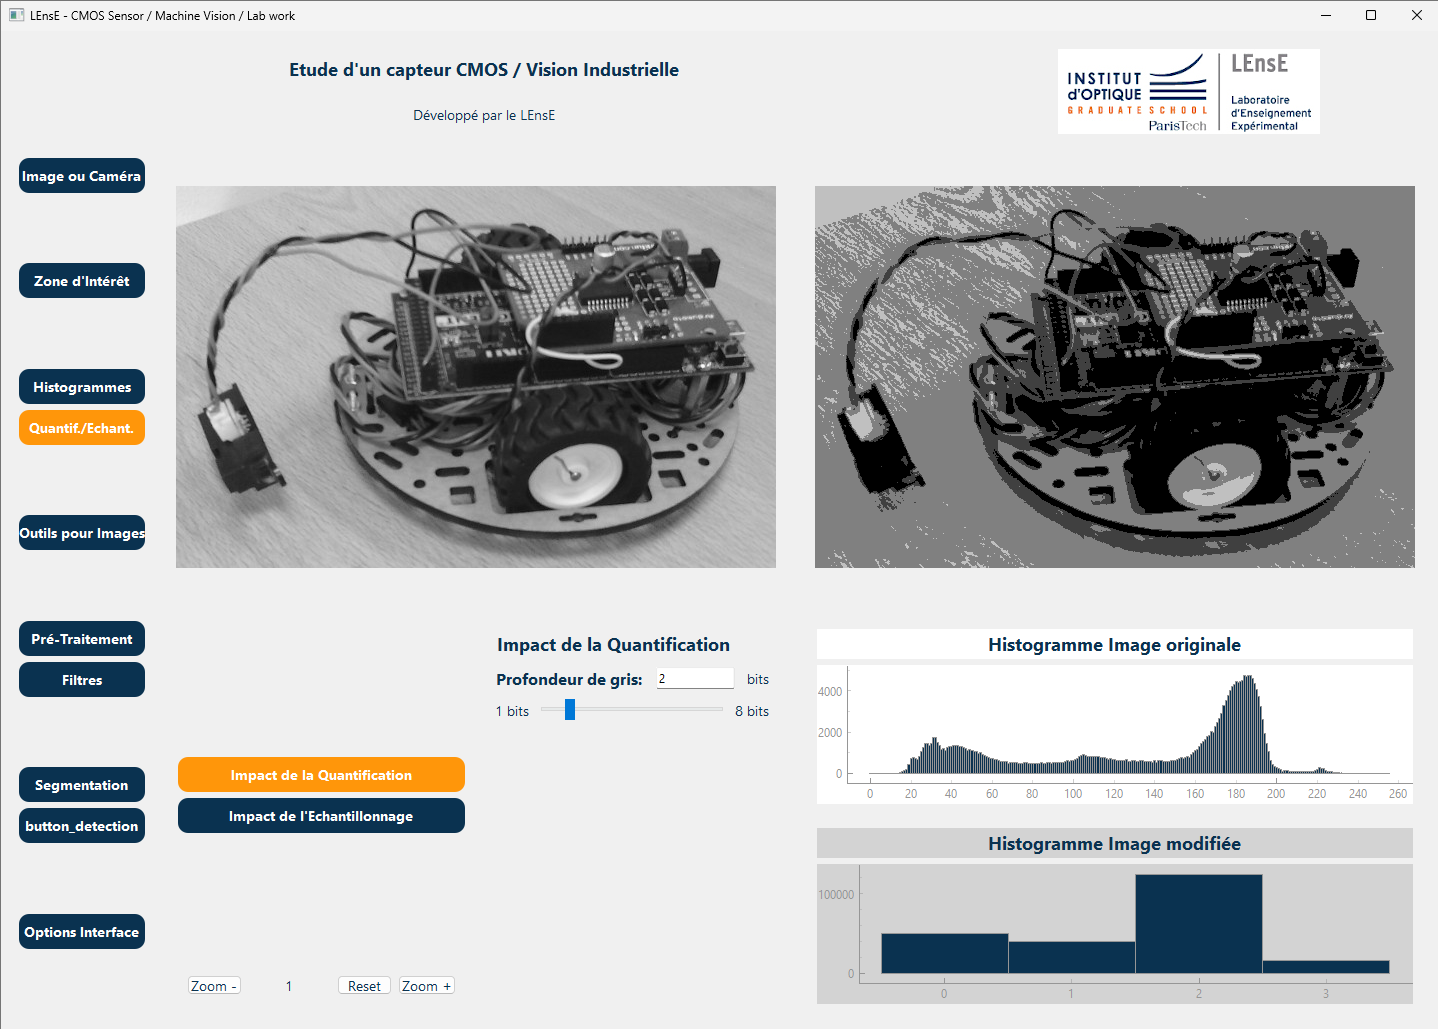
\includegraphics[width=0.9\textwidth]{./images/camera_gui.png}
\end{center}


\Manip Ouvrir la première caméra disponible dans l'onglet \textsc{Image ou Caméra} / \textsc{Sélectionner une caméra} / \textsc{Ouvrir la première caméra}.

\subsection{Eclairage et zone d'intérêt}

\Manip Allumer l'éclairage annulaire du banc (trois couleurs). 

\Quest Quelle couleur d'éclairage obtient-on ?

\Manip Placer un objet (un cube de couleur par exemple) dans le champ de la caméra.

\Manip Ajuster la zone d'intérêt (ou \textit{Area of Interest} - AOI) à l'aide de l'onglet \textsc{Zone d'Intérêt} pour ne sélectionner qu'une partie de l'image autour de l'objet.

\Quest Que pouvez-vous dire des deux histogrammes affichés ? Quelles sont les valeurs minimale et maximale prises par les pixels de la caméra ? Quelle est alors la résolution de la caméra utilisée ?

\medskip

\Quest A quoi servent les deux bagues présentes sur l'objectif ?


\noindent \rule{\linewidth}{1pt}

\textit{\textbf{Pour la suite du TP, on s'assurera de prendre une zone d'intérêt à peu près centrée dans l'image et d'une taille d'environ 500 par 500 pixels.}}


\newpage
%%%%%%%%%%%%%    Etape 1
\section{Etape 1 / Décrire le rôle des principales caractéristiques d'une caméra CMOS}

\begin{center} \textbf{\textit{Temps conseillé : 30 min}} \end{center}


\subsection{Temps d'intégration}

\Manip Dans l'onglet \textsc{Image ou Caméra}, sélectionner un \textit{Black Level} de 0. Modifier le temps d'intégration de la caméra.

\Quest Que constatez-vous sur l'histogramme de l'image ? Sur la moyenne et l'écart-type de la répartition de la luminosité des pixels ?

\Manip Placer un cache devant la caméra (ou Prévoir une caméra annexe avec cache - pour éviter d'enlever l'objectif et mettre un cache...) pour vous placer dans l'obscurité.

\Quest La répartition de la luminosité perçu par chaque pixel est-elle uniforme ? Que pouvez-vous en conclure ?


\subsection{Black Level}

\Manip Dans l'obscurité, relever l'histogramme de l'image ainsi que la moyenne et l'écart-type de la répartition de la luminosité des pixels pour différentes valeurs du \textit{black level} : 0, 5, 10, 15.

\Quest Que peut-on conclure de l'intérêt du black level ?

\subsection{Echantillonnage et quantification}

\Manip Replacer l'objectif sur la caméra. Placer des objets dans le champ de la caméra. Sélectionner une zone d'intérêt d'environ 500 pixels par 500 pixels autour de l'objet à visualiser. Ajuster le temps d'intégration pour obtenir une image non saturée avec un éclairage blanc. 

\Manip Dans la section \textsc{Quantif./Echant.}, modifier la profondeur de quantification des informations. 

\Quest Que peut-on conclure sur l'effet de la quantification sur l'image ? Vous pourrez vous appuyer sur l'histogramme pour analyser le résultat.

\Manip De la même façon, dans la section \textsc{Quantif./Echant.}, modifier le nombre de pixels de sous-échantillonnage. 

On parle ici d'un phénomène de \textbf{binning}. La résolution de l'image est "dégragée" numériquement dans ce cas et les nouveaux pixels affichés sont la moyenne de N x N pixels de l'image initiale.

\textit{Dans le cas présent, ce phénomène peut simuler le changement de résolution de la caméra sur l'acquisition d'une image numérique.}

\Quest Que peut-on conclure sur l'effet de la résolution de la caméra sur l'image ? Vous pourrez vous appuyer sur l'histogramme pour analyser le résultat.


\newpage
%%%%%%%%%%%%%    Etape 2
\section{Etape 2 / Analyser l'impact des outils de base de la manipulation d'images}

\begin{center} \textbf{\textit{Temps conseillé : 60 min}} \end{center}

Dans cette section, nous allons nous intéresser à quelques fonctionnalités permettant de \textbf{manipuler des images} pour les rendre utilisables : suppression du bruit, seuillage, amélioration du contraste...

\subsection{Contraste et Luminosité}

\Manip Placer un objet dans le champ de la caméra. Sélectionner une zone d'intérêt d'environ 500 pixels par 500 pixels autour de l'objet à visualiser. Ajuster le temps d'intégration pour obtenir un histogramme dont le pixel maximum a une valeur de l'ordre des 2/3 de la valeur maximale de la caméra. 

\Manip Dans la section \textsc{Pré-Traitement}, puis sous-section \textsc{Contraste / Luminosité}, modifier les valeurs de contraste et de luminosité de l'image.

\Quest Quelles sont les opérations mathématiques réalisées sur les pixels par ces deux fonctionnalités ? Vous pourrez vous appuyer sur les histogrammes des images brutes et modifiées pour analyser vos résultats.

\Manip Dans la sous-section \textsc{Amélioration du Contraste}, tester l'effet des deux curseurs.

\Quest Proposer une interprétation de l'opération effectuée sur chacun des pixels.


\subsection{Seuillage}

\Manip Dans la section \textsc{Pré-Traitement}, puis sous-section \textsc{Seuillage}, sélectionner le seuillage \textsl{Normal} et modifier la valeur du seuil.

\Quest Que pouvez-vous conclure sur l'intérêt du seuillage ? Vous pourrez essayer avec des objets de taille, de forme et de couleurs différentes.

\Manip Tester également le mode \textsl{Inversé} et \textsl{Double}.

\Quest Que pouvez-vous conclure sur ces deux modes ?
 

\subsection{Filtrage}

\Manip Dans la section \textsc{Filtres}, puis sous-section \textsc{Filtre de lissage}, sélectionner le filtre \textsl{Blur Moyen} et un noyau de taille 15.

\Quest Que se passe-t-il sur l'image ? Vous pourrez également vous appuyer sur la différence entre l'image de base et l'image modifiée, en cliquant sur l'option \textsl{Image - Effet}, pour analyser les effets sur l'image.

\Quest Quel est l'effet de la taille du noyau sur le filtrage ?

\Quest Qu'en est-il avec le filtre de type \textsl{Médian} ? 

\medskip

\textit{Les aspects théoriques liés au filtrage de données (signaux et images) sont abordés dans les modules \textsc{Maths et Signal} (semestre 5) et \textsc{Traitement du Signal} (semestre 6).}

\textit{La mise en oeuvre de ces filtres sur des images sera abordée en TD de ce module et également dans des modules de traitement d'images dans vos prochaines années de formation.}


\newpage
%%%%%%%%%%%%%    Etape 3
\section{Etape 3 / Analyser l'impact du choix de la couleur de l'éclairage}

\begin{center} \textbf{\textit{Temps conseillé : 60 min}} \end{center}

L'acquisition d'image réalisée par l'interface est monochrome. Il est toutefois possible de détecter des couleurs dans les objets à analyser en jouant sur le choix de l'éclairage et sa couleur.


\subsection{Acquisition à des longueurs d'onde différentes}

Vous avez à votre disposition plusieurs objets de couleurs différentes.

\begin{center}
	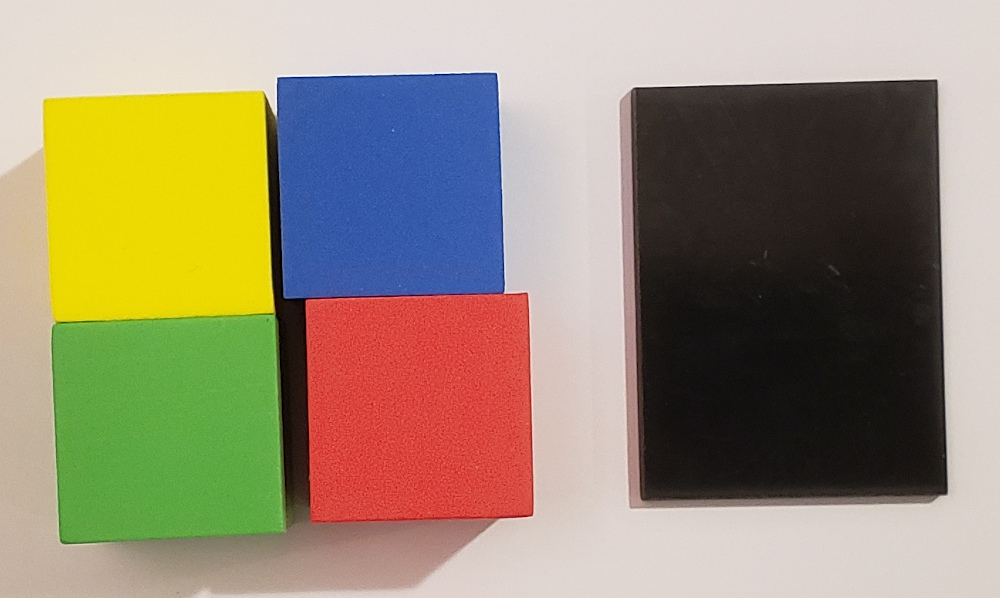
\includegraphics[width=0.4\textwidth]{images/cubes.jpg}
\end{center}


\Manip Placer les cubes de 4 couleurs différentes dans le champ de la caméra. Placer également la surface plane noire dans le champ.

\Manip Eclairer successivement la scène en rouge, puis en bleu, puis en vert. Visualiser les images acquises ainsi que les histogrammes associées.

\textit{Il est préférable de faire ces analyses dans une environnement sombre, voir dépourvu de tout éclairage parasite.}

\Quest A partir des histogrammes, proposer une méthode de détection des couleurs des objets.

\Manip Tester votre méthode. Faire valider par un$\cdot$e enseignant$\cdot$e.

\medskip

\Manip Placer à présent la feuille qui présente 3 carrés de couleurs différentes et un dessin.

\begin{center}
	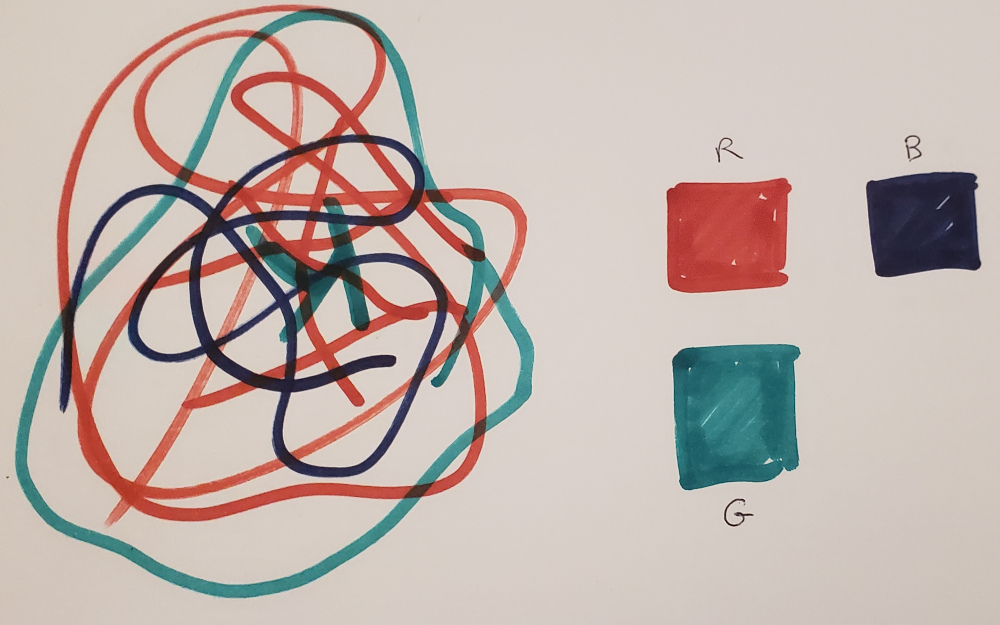
\includegraphics[width=0.4\textwidth]{images/dessin.jpg}
\end{center}

\Quest Proposer une méthode de détection de ces couleurs, afin de n'extraire qu'un des carrés.

\Manip Tester votre méthode. Faire valider par un$\cdot$e enseignant$\cdot$e.

\Quest Quelle lettre se cache dans votre dessin ? 

\textit{Vous pouvez également demander l'oeuvre de Thierry A. et rechercher la lettre mystère...}

\subsection{Filtrage optique}

Une autre solution est l'utilisation de filtre optique. Vous avez à votre disposition 3 filtres (R, G, B).

\Manip Tester les différentes combinaisons filtre et éclairage en analysant les objets de couleurs dans le champ de la caméra.

\Quest Est-il possible de renforcer la détection des couleurs des objets par ce principe ?

\newpage
%%%%%%%%%%%%%    Etape 4
\section{Etape 4 / Détecter des objets dans une image}

\begin{center} \textbf{\textit{Temps conseillé : 60 min}} \end{center}

On se propose de détecter les \textbf{veines de nos doigts} à l'aide de la caméra et de l'éclairage présent sur le banc. Pour cela, nous allons devoir trouver une spécificité dans la couleur de l'objet que l'on cherche à identifier par rapport au reste de la scène (le sang qui coule dans nos veines est plutôt de couleur rouge...).

\begin{center}
	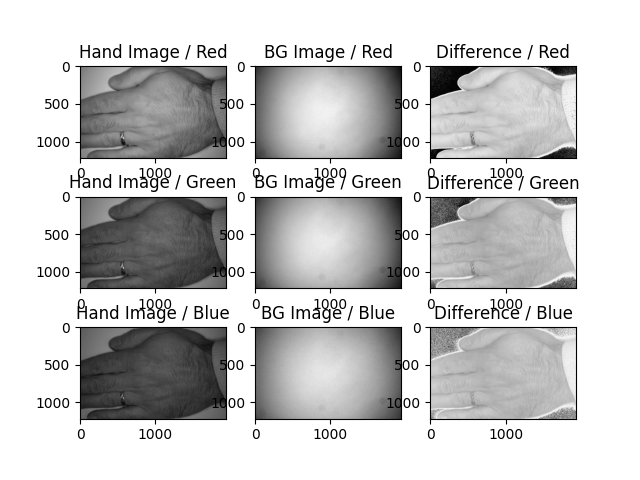
\includegraphics[width=0.4\textwidth]{images/hands.png}
\end{center}

On peut montrer expérimentalement que l'image résultante ($I$) du calcul suivant permet d'obtenir une image relativement exploitable :

$$I = \frac{I_R}{\sqrt{I_G^2 + I_B^2}}$$

où $I_X = X_{main} - X_{blanc}$ correspond à l'image de la main prise en éclairage R-G-B (rouge, vert ou bleu) sur un fond blanc, à laquelle on a retranché le fond blanc prise dans les mêmes conditions d'éclairage et de temps d'exposition.

\subsection{Protocole}

\textbf{L'ensemble des images devront être prises dans les mêmes conditions géométriques (vous ne devrez pas bouger ni le fond blanc ni votre main) et d'acquisition (temps d'intégration notamment).}

On se placera dans la section \textsc{Histogrammes}, sous-section \textsc{Répartition spatiale} de l'interface de pilotage. Cette section permet de régler le temps d'intégration mais également de sauvegarder une image au format PNG.

\medskip

Le protocole proposé est le suivant :

\begin{itemize}
	\item Régler le temps d'intégration pour ne pas saturer l'image mais garantir une bonne dynamique d'acquisition, quelques soient les conditions d'éclairage (R, G, B). \textit{Il faudra également vérifier cette dynamique sur fond blanc et en présence de votre main.}
	\item Acquérir les images sur fond blanc \textbf{sans} l'objet à analyser avec un éclairage rouge, puis bleu, puis vert et les sauvegarder indépendamment au format PNG.
	\item Acquérir les images sur fond blanc \textbf{avec} l'objet à analyser avec un éclairage rouge, puis bleu, puis vert et les sauvegarder indépendamment au format PNG.
	\item Ouvrir les images avec un script (Python par exemple).
	\item Réaliser le traitement proposé précédemment.
	\item Afficher l'image résultante.
\end{itemize}

\newpage
\subsection{Ouverture d'une image avec OpenCV}

Pour ouvrir les images, nous allons utiliser la bibliothèque \textbf{OpenCV} (plus de détails dans la séance 2 de ce TP). Nous utiliserons la version développée pour le langage Python.

Pour installer cette extension sous Python, il faut exécuter la commande suivante dans un terminal (ou Invite de commande sous Windows) :

\begin{lstlisting}
pip install opencv-python
\end{lstlisting}

\medskip

Si l'on souhaite ouvrir l'image \textsl{test.png} stockée dans le même que votre script en Python, à l'aide de la bibliothèque OpenCV et l'afficher, il faut utiliser les instructions suivantes :

\begin{lstlisting}
import cv2
from matplotlib import pyplot as plt

grayscale_image = cv2.imread('test.png', cv2.IMREAD_GRAYSCALE)
plt.imshow(grayscale_image, cmap='gray')
plt.show()
\end{lstlisting}

L'objet \textsl{grayscale\_image} est une matrice en deux dimensions, issue de la bibliothèque \textsl{Numpy}. Il est alors possible de faire des calculs sur cette matrice : moyenne, somme, addition et autres opérations mathématiques avec d'autres matrices...).

Il sera également possible d'appliquer d'autres fonctionnalités de pré-traitement ou de filtrage. Ces notions seront abordées dans la séance de TP suivante.


\subsection{Traitement avec OpenCV}

\Manip Réaliser les premières étapes du protocole afin de prendre des images exploitables du fond blanc choisi dans les 3 conditions d'éclairage proposées (R, G et B) ainsi que les images d'une main dans les mêmes conditions d'éclairage et d'acquisition pour la caméra.

\Manip Réaliser un script Python permettant d'ouvrir et d'afficher les 6 images.

\Manip Ajouter à ce script la possibilité de calculer l'image résultante du traitement proposé pour détecter les veines.

Il pourra être intéressant de calculer le logarithme de l'image résultante et d'afficher le résultat. Afin d'isoler plus facilement les pixels intéressants, vous pourrez utiliser l'interface de la caméra en chargeant l'image du logarithme de $I$ et utiliser le seuillage double pour isoler les objets intéressants...

\Quest Est-ce concluant ? Vous pourrez répéter ces étapes afin d'obtenir une meilleure qualité d'image (en jouant sur le temps d'intégration notamment).

\begin{center}
	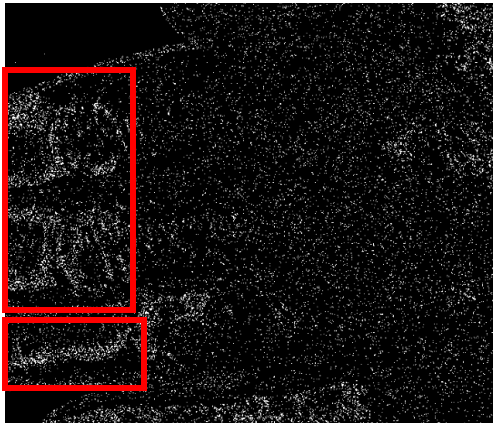
\includegraphics[width=0.3\textwidth]{images/blood_detect.png}
\end{center}




\newpage
\strut % empty page
%%%%%%%%%%%%%%%%%%%%%%%%%%%%%%%%%%%%%%%%%%%%%%%%
%%%%%%%%%%%%%    Séance 2 détaillée
\begin{minipage}[c]{.25\linewidth}
	
\includegraphics[width=4cm]{images/Logo-LEnsE.png}
\end{minipage} \hfill
\begin{minipage}[c]{.4\linewidth}

\begin{center}
\vspace{0.3cm}
{\Large \textsc{Interfaçage Numérique}}

\medskip

6N-047-SCI \qquad \textbf{\Large Bloc Caméra}

\end{center}
\end{minipage}\hfill

\vspace{0.5cm}

\noindent \rule{\linewidth}{1pt}

{\noindent\Large \rule[-7pt]{0pt}{30pt} \textbf{Séance 2} / Manipulation d'images (OpenCV) et filtrage} 

\noindent \rule{\linewidth}{1pt}

Lors de cette séance, vous devrez écrire vos propres scripts en \textbf{Python} (avec l'IDE PyCharm par exemple) permettant de réaliser des opérations de base de manipulation d'images, à l'aide notamment de la célèbre bibliothèque \textbf{OpenCV}.

\section{Ressources}

Un tutoriel sur les bases d'OpenCV est disponible à l’adresse suivante : 

\href{https://iogs-lense-training.github.io/image-processing/}{https://iogs-lense-training.github.io/image-processing/}

Un \textbf{kit d'images} est disponible sur le site du LEnsE dans la rubrique \textit{Année / Première Année / Interfaçage Numérique S6 / Bloc Images et OpenCV / Kit d'images}. 


%%%%%%%%%%%%%    Etape 1
\section{Etape 1 / Ouvrir une image sous OpenCV}

\begin{center} \textbf{\textit{Temps conseillé : 20 min}} \end{center}

\begin{mdframed}[style=sidebar,frametitle={}]
Notions : \href{https://iogs-lense-training.github.io/image-processing/contents/opencv.html#open-an-image
}{\textit{Open an image}} - \href{https://iogs-lense-training.github.io/image-processing/contents/opencv.html#display-an-image
}{\textit{Display an image}}
\end{mdframed}

\Manip Créer un nouveau projet sous PyCharm.

\Manip Impoter la bibliothèque \textbf{OpenCV2} (\textit{cv2}).

\medskip

\textit{Pour la suite, il est nécessaire de placer \textbf{tous les fichiers dans le même dossier} : votre script Python, les
différentes images et les bibliothèques de fonction (fichier \textsl{images\_manipulation.py})}

\Manip Ouvrir l'image \textsl{robot.jpg} du kit d'images fourni, au format RGB.

\Quest Quelle est la taille de l'image ? Quel est le type de données d'un élément ?

\Manip Ouvrir l'image \textsl{robot.jpg} du kit d'images fourni, en niveau de gris.

\Quest Quelle est la taille de l'image ? Quel est le type de données d'un élément ?


%%%%%%%%%%%%%    Etape 2
\section{Etape 2 / Calculer l'histogramme d'une image et l'afficher}

\begin{center} \textbf{\textit{Temps conseillé : 20 min}} \end{center}

\begin{mdframed}[style=sidebar,frametitle={}]
Notions : \href{https://iogs-lense-training.github.io/image-processing/contents/opencv.html#histogram-of-an-image}{\textit{Calculate the histogram}}
\end{mdframed}

\Manip Calculer l'histogramme de l'image précédente et l'afficher.

\medskip

\textit{Il peut être intéressant de \textbf{créer une fonction qui affiche automatiquement l'histogramme} d'une image à partir de ses données. Elle sera très utile dans la suite du TP pour voir l'impact des effets appliqués sur les images.}


%%%%%%%%%%%%%    Etape 3
\section{Etape 3 / Améliorer numériquement la qualité d'une image}

\begin{center} \textbf{\textit{Temps conseillé : 20 min}} \end{center}

\begin{mdframed}[style=sidebar,frametitle={}]
Notions : \href{https://iogs-lense-training.github.io/image-processing/contents/opencv.html#enhance-the-image-contrast-and-brightness
}{\textit{Enhance Contrast/Brightness}}
\end{mdframed}

Pour modifier le contraste et la luminosité d'une image, il faut appliquer une transformation linéaire \textbf{à chaque pixel} de l'image pouvant être exprimé mathématiquement comme suit :

$$P_{new} = \alpha \cdot P_{old} + \beta$$

où $\alpha$ est le facteur de contraste. Une valeur supérieure à 1 augmente le contraste, tandis qu'une valeur entre 0 et 1 le réduit.

$\beta$ est l'offset de luminosité. Une valeur positive rend l'image plus lumineuse, tandis qu'une valeur négative l'assombrit.

\medskip

On utilisera la fonction \textsl{cv2.convertScaleAbs()} pour modifier le contraste et la luminosité de l'image.

\bigskip

\Manip Ouvrir l'image \textsl{robot.jpg} du kit d'images fourni, en niveau de gris.

\Manip Modifier le contraste de l'image et comparer les histogrammes de l'image originale et de la version modifiée pour différente valeur de $\alpha$.

\Manip Modifier la luminosité de l'image et comparer les histogrammes de l'image originale et de la version modifiée pour différente valeur de $\beta$.


%%%%%%%%%%%%%    Etape 4
\section{Etape 4 / Appliquer un filtre moyenneur sur une image}

\begin{center} \textbf{\textit{Temps conseillé : 90 min}} \end{center}

La transformation précédente ne prend pas en compte les pixels voisins. Il est pourtant intéressant dans de nombreuses situations de capturer des relations spatiales entre les pixels.

Les filtres prenant en compte les pixels voisins exploitent les relations locales dans une image, ce qui est crucial pour des tâches comme la suppression de bruit, la détection de contours, l'extraction de caractéristiques, et l'amélioration de la qualité visuelle. Travailler sur des pixels isolés limite l'analyse à des informations ponctuelles, tandis que considérer les voisins permet une compréhension plus riche et contextuelle de l'image.

\subsection{Eléments structurants ou noyau}

Un \textbf{élément structurant} (ou noyau) est une petite matrice (généralement de taille et de forme prédéfinies, comme un carré, un disque, une ligne, etc.) qui sert de sonde pour inspecter et modifier les pixels d'une image.  

\begin{center}
	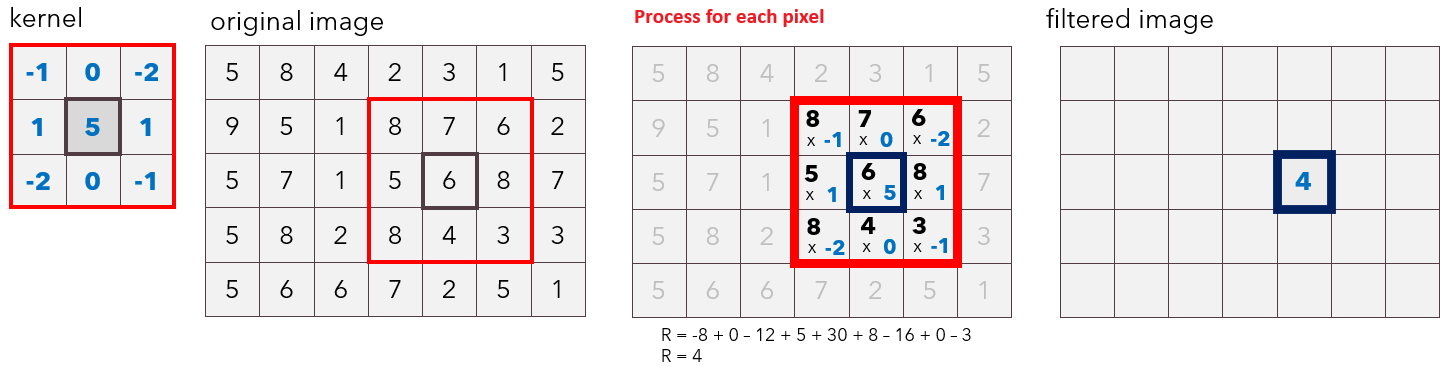
\includegraphics[width=\textwidth]{images/kernel.png}
\end{center}

Les éléments structurants jouent un rôle clé en traitement d'image, notamment dans les opérations de morphologie mathématique. Ces opérations sont principalement utilisées pour analyser et traiter des images binaires ou en niveaux de gris en modifiant leurs formes ou en extrayant des structures spécifiques.


\subsection{Filtre moyenneur gaussien}

\begin{mdframed}[style=sidebar,frametitle={}]
Notions : \href{https://iogs-lense-training.github.io/image-processing/contents/opencv_blur.html#blur-with-opencv
}{\textit{Blur with OpenCV}}
\end{mdframed}

\Manip Créer un nouveau projet sous PyCharm.

\Manip Impoter la bibliothèque \textbf{OpenCV2} (\textit{cv2}).

\Manip Ouvrir l'image \textsl{bricks2.jpg} du kit d'images fourni, en niveau de gris.

\Manip Appliquer un filtre gaussien (fonction \textsl{cv2.GaussianBlur()}) sur l'image précédente, de taille 5 x 5 pixels.

\Manip Afficher les deux images pour les comparer.

\Quest Comment peut-on montrer de manière objective les modifications apportées à l'image ? 

\Manip Mettre en oeuvre la méthode proposée.

\medskip

On se propose d'utiliser la fonction \textsl{compare\_blur\_fft()} fournie dans le fichier \textsl{images\_manipulation.py} pour comparer l'effet. 

Ce fichier est disponible sur le site du LEnsE dans la rubrique \textit{Année / Première Année / Interfaçage Numérique S6 / Bloc Images et OpenCV / Répertoire vers codes à tester}.

\Manip Tester cette fonction sur l'image précédente.

\Quest Etudier cette fonction. Quelles méthodes sont utilisées pour comparer les images ?

\Quest Quelle est la fonction réalisée par le filtre précédent ?

\medskip

On cherche à présent à voir l'impact du noyau sur l'image finale.

\Manip Tester la fonction précédente avec des noyaux de taille différente et comparer les résultats à la fois sur l'image obtenue mais également sur la transformée de Fourier.

\Quest Que pouvez-vous conclure sur l'impact de la taille du noyau ?


\subsection{Bruit sur une image}

On se propose d'étudier la fonction \textsl{generate\_gaussian\_noise\_image()} fournie dans le fichier \textsl{images\_manipulation.py}.

\Manip Tester l'exemple fourni dans le fichier \textsl{noise\_test1.py}.

\Quest Comment vérifier la distribution du bruit généré par cette fonction ?

\medskip

On se propose d'étudier la fonction \textsl{generate\_uniform\_noise\_image()} fournie dans le fichier \textsl{images\_manipulation.py}.

\Manip Tester l'exemple fourni dans le fichier \textsl{noise\_test2.py}.

\Quest La distribution du bruit généré par cette fonction est-elle uniforme ?

\Manip A l'aide de la fonction \textsl{generate\_gaussian\_noise\_image\_percent()}, générer un bruit gaussien de moyenne 30 et d'écart-type 20 sur 10\% de l'image \textsl{robot.jpg} ouverte précédemment en nuance de gris. Visualiser le résultat.

\medskip

\textit{Il peut-être nécessaire de normaliser les images bruitées afin que les \textbf{données entières} de chaque pixel soient comprises \textbf{entre 0 et 255}, afin que les images puissent être affichées correctement.} 

\Manip Tester la fonction \textsl{compare\_blur\_fft()} fournie dans le fichier \textsl{images\_manipulation.py} et comparer les résultats à la fois sur l'image obtenue mais également sur la transformée de Fourier.


%%%%%%%%%%%%%    Etape 5
\section{Etape 5 / Appliquer un filtre passe-haut sur une image}

\begin{center} \textbf{\textit{Temps conseillé : 60 min}} \end{center}

Le \textbf{filtre moyenneur} précédent permet de conserver les \textbf{éléments à basse fréquence spatiale} dans l'image. C'est une méthode intéressante pour supprimer des bruits ponctuels (des éléments isolés et donc "rapides"). Il est également possible en choisissant un autre élément structurant de réaliser l'opération complémentaire qui supprime le fond continu et ne conserve que les transitions de fréquence spatiale élevée (bords d'un objet par exemple).

\medskip

Il est possible d'utiliser la fonction \textsl{cv2.filter2D()} pour appliquer un noyau particulier sur une image.

\subsection{Opérateur de Roberts}

L'opérateur de Roberts est l'un des premiers filtres de \textbf{détection de contours}. Il repose sur la convolution avec deux petits noyaux 2x2, conçus pour approximer les dérivées en diagonale de l'image.

Les noyaux de convolution sont les suivants :

$$K_x = \begin{bmatrix}
+1 & 0 \\
0 & -1
\end{bmatrix},
\quad
K_y =
\begin{bmatrix}
0 & +1 \\
-1 & 0
\end{bmatrix}.
$$

Il est alors possible de calculer l'amplitude du gradient par l'opération suivante: 

$$\text{Amplitude} = \sqrt{G_x^2 + G_y^2}$$ où $G_x$ est le résultat de la convolution de l'image par le noyau $K_x$ et $G_y$ le résultat de la convolution de l'image par le noyau $K_y$.

Une forte amplitude indique un contour ou un bord marqué. Une faible amplitude indique une région où l'intensité est relativement constante.

\medskip

\Manip Ecrire un script qui permet d'appliquer cette opération sur l'image \textsl{bricks2.jpg} du kit d'images fourni, en niveau de gris.

\Manip Visualiser l'image originale, le résultat du filtrage selon X et le résultat du filtrage selon Y.

\Quest Que pouvez-vous conclure sur l'effet de ce filtre ?

\subsection{Opérateur de Sobel}

L'opérateur de Sobel permet de réaliser une opération similaire à celui de Roberts, mais en étant moins sensible aux bruits dans l'image, puisqu'il se base sur un noyau plus large et ainsi lisse l'image dans la direction perpendiculaire au gradient mesuré.

Les noyaux de convolution sont les suivants :

$$G_x = \begin{bmatrix}
-1 & 0 & 1 \\
-2 & 0 & 2 \\
-1 & 0 & 1 
\end{bmatrix},
\quad
G_y =
\begin{bmatrix}
-1 & -2 & -1 \\
0 & 0 & 0 \\
1 & 2 & 1 
\end{bmatrix}.
$$

De la même façon que précédemment, on peut calculer l'amplitude du gradient par l'opération suivante : 

$$\text{Amplitude} = \sqrt{G_x^2 + G_y^2}$$ où $G_x$ est le résultat de la convolution de l'image par le noyau $K_x$ et $G_y$ le résultat de la convolution de l'image par le noyau $K_y$.

\medskip

\Manip Ecrire un script qui permet d'appliquer cette opération sur l'image \textsl{bricks2.jpg} du kit d'images fourni, en niveau de gris.

\Manip Visualiser l'image originale, le résultat du filtrage selon X et le résultat du filtrage selon Y.

\Quest Que pouvez-vous conclure sur l'effet de ce filtre ?

%%%%%%%%%%%%%    Etape 6
\section{Etape 6 / Appliquer un filtre par l'intermédiaire de la transformée de Fourier}

\begin{center} \textbf{\textit{Temps conseillé : 30 min}} \end{center}

On s'intéresse ici à la \textbf{transformée de Fourier discrète en deux dimensions} permettant de représenter l'image dans le domaine fréquentiel, plutôt que dans le domaine spatial.

\Manip Ouvrir l'image \textsl{robot.jpg} du kit d'images fourni, en niveau de gris.

\Manip Calculer la transformée de Fourier discrète de cette image à l'aide de la fonction \textsl{fft2()} de la bibliothèque \textbf{Numpy / FFT}. Afficher l'image et sa transformée de Fourier. \textit{Pensez à utiliser la fonction fftshift...}

\medskip

On se propose d'utiliser la fonction \textsl{circular\_mask()} fournie dans le fichier \textsl{images\_manipulation.py} pour appliquer un masque sur la transformée de Fourier de l'image. 

Ce fichier est disponible sur le site du LEnsE dans la rubrique \textit{Année / Première Année / Interfaçage Numérique S6 / Bloc Images et OpenCV / Répertoire vers codes à tester}.

\Manip Appliquer un masque circulaire sur la transformée de Fourier de l'image, à l'aide de la fonction \textsl{circular\_mask()}. Afficher le résultat.

\Manip Calculer l'image résultante à l'aide de la fonction \textit{ifft2()} de la bibliothèque \textbf{Numpy / FFT}. Afficher l'image résultante et la comparer à l'image originale.

\medskip

\Manip Ecrire et tester une fonction permettant de réaliser un masquage rectangulaire sur une image, dont on pourra préciser la largeur et la longueur, ainsi que le barycentre du rectangle (point d'intersection des diagonales).

\Quest Que se passe-t-il lorsque vous appliquez un masque rectangulaire (dont la largeur et la longueur sont différentes) sur une image ? Qu'en est-il d'un masque circulaire ?


%%%%%%%%%%%%%%%%%%%%%%%%%%%%%%%%%%%%%%%%%%%%%%%%
%%% RESSOURCES COMPLEMENTAIRES	

\newpage
\begin{center}
	\begin{minipage}{2.5cm}
	\begin{center}
		
\includegraphics[width=5cm]{images/Logo-LEnsE.png}
	\end{center}
\end{minipage}\hfill
\begin{minipage}{10cm}
	\begin{center}
	\textbf{Institut d'Optique Graduate School }\\[0.1cm]
    \textbf{Interfaçage Numérique}


	\end{center}
\end{minipage}\hfill


\vspace{2cm}


{\Large \bfseries \textsc{Interfaçage Numérique}} \\[0.5cm]
{\large \bfseries Travaux Pratiques} \\[0.2cm]
Semestre 6

\vspace{1cm}

% Title
\rule{\linewidth}{0.4mm} \\[0.4cm]
{ \Large \bfseries\color{violet_iogs} Ressources \\[0.4cm] }
\rule{\linewidth}{0.4mm} \\[1cm]
{\large Bloc Caméra}

\end{center}

\vspace{3cm}



\textbf{\large Liste des ressources}
\begin{itemize}
	\item \hyperref[doc:image_proc]{Camera and sensor / Key concepts}
\end{itemize}

\vfill

\newpage
\strut % empty page


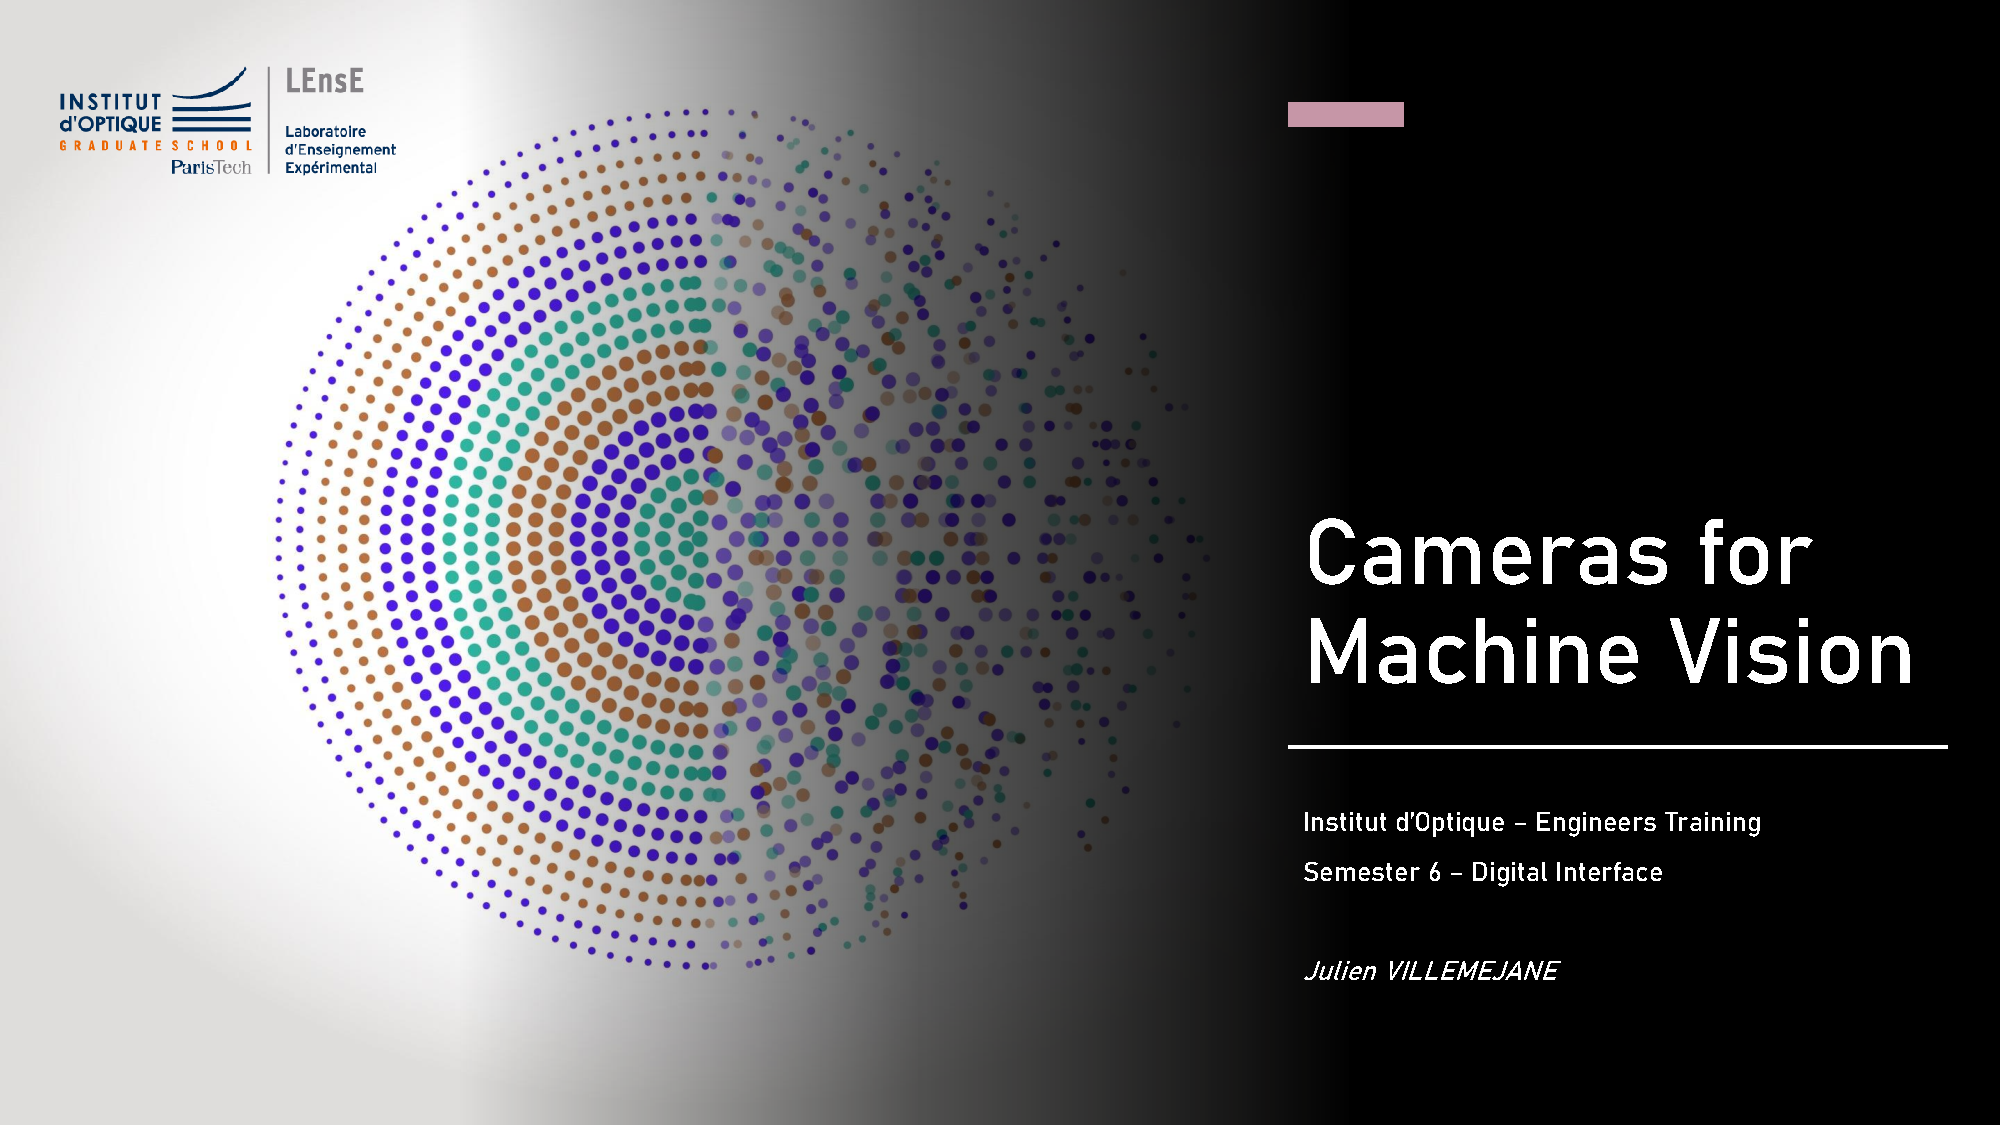
\includepdf[pages={1,3}, nup=1x2, pagecommand={\section{\texorpdfstring{\hspace{-1em}}{Camera and sensor}}}\label{doc:image_proc}]{../docs/Cameras.pdf}
\includepdf[pages={7,10-14,16,19,22,23,24,25,8}, nup=1x2]{../docs/Cameras.pdf}


\end{document}


